%----------------------------------------------------------------------------------------
%----------------------------------------------------------------------------------------
%----------------------------------------------------------------------------------------
%DATA
%----------------------------------------------------------------------------------------
%----------------------------------------------------------------------------------------
%----------------------------------------------------------------------------------------

\section{Study sample} %%or sample study?!
\label{Sec: data_SOMN}

Our study includes 10 regions in M31 (Fig.~\ref{fig: regions in m31}) and 8 regions in M101 (Fig.~\ref{fig: regions in m101}). 
These specific regions were chosen for the availability of \Spitzer/IRS 5 - 15$\mu$m  spectroscopy covering PAHs emission.
Besides PAH bands strengths, for each galaxy, we use spectroscopic and photometric observations as well as their derived properties, such as SFR, stellar mass, dust luminosity (L$_{\rm dust}$), and mass, metallicity, and gas mass.
Table~\ref{tab: data} shows the full list of data for both M31 and M101.
All data were divided by the area of their region (in arcsec$^2$), to remove the distance factor from the data and compare values across galaxies.
Since the spatial resolution of the observations varies from $<1$\arcsec to 60\arcsec $\times$ 90 \arcsec, any attempt to match resolution would have caused a loss of information in some of the input quantities (e.g. the spectroscopic data).
In this project we used flux per unit area, which the convolution methods conserve~\citep{Aniano12}, as the input data.
Therefore, we did not perform any resolution matching and used data at their original resolution. %PB: Need to discuss these last few sentences; not sure I understand what you're saying.


\import{../sections/tables/}{tab_data.tex}

\begin{figure}
  \begin{subfigure}[b]{0.5\textwidth}
        \centering
    %\centering
        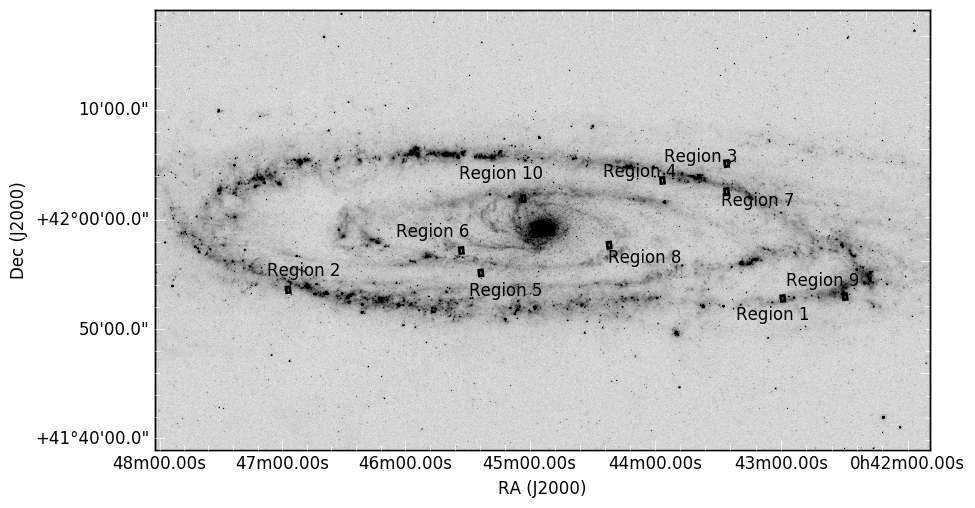
\includegraphics[width=0.97\textwidth]{../images0.01/M31/M31.png}
        \caption{MIPS~24 image of M31, with position of 10 regions that we studies.}
        \label{fig: regions in m31}
    \end{subfigure}
    \hfill
    \begin{subfigure}[b]{0.5\textwidth}
        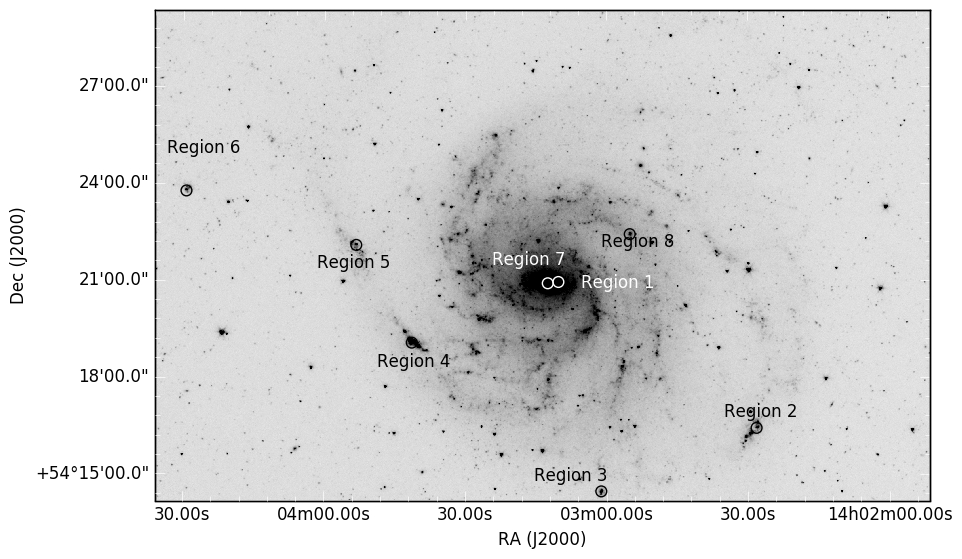
\includegraphics[width=\textwidth]{../images0.01/M101/M101.png}
        \caption{IRAC1 image of M101, with position of our 8 regions that we studies.}
    \label{fig: regions in m101}
    \end{subfigure}
    \caption{Position of the data in M31 (up) and M101 (down).}
\end{figure}

%   \begin{figure}
%     \subfloat[MIPS 24~$\mu$m image of M31~\citep{Gordon06}, with position of 10 regions from~\cite{Dim15} \label{fig: regions in m31}]{
%       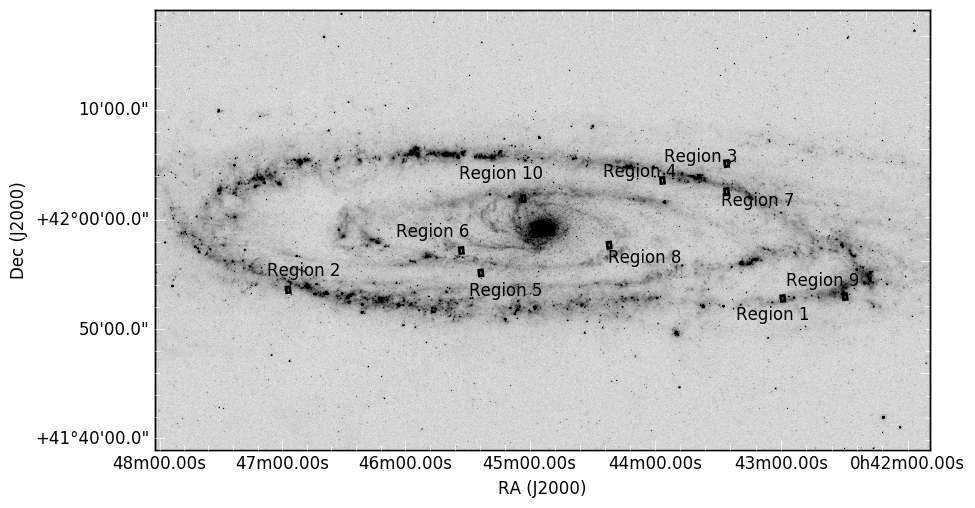
\includegraphics[width=0.5\textwidth]{../images0.01/M31/M31.png}
%     }
%     \hfill
%     \subfloat[IRAC 3.6~$\mu$m image of M101~\citep{Dale09}, with position of 8 regions.\label{fig: regions in m101}]{
%       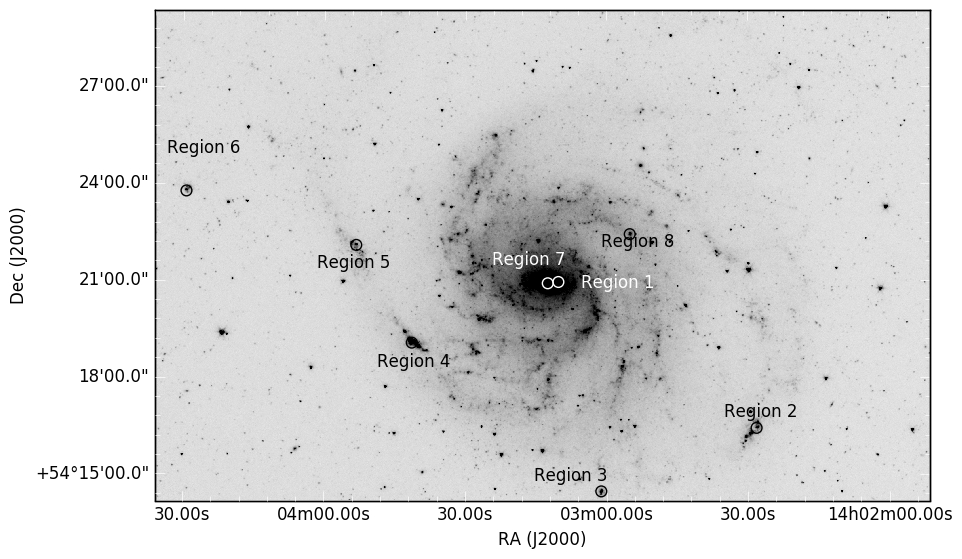
\includegraphics[width=0.5\textwidth]{../images0.01/M101/M101.png}}
%     \caption{Position of regions that the input data for SOM that obtained from there in M31 (up) and M101 (down).}
%     \label{fig:dummy}
%   \end{figure}

    \subsection{M31 observations}
     \label{Sec: data_M31_SOMN} 
     
     \cite{Dim15} used {\it Spitzer}/IRS observations to study PAHs in 10 regions chosen to span a range of mid-infrared flux ratios in M31 (Fig.~\ref{fig: regions in m31}). 
     Fluxes and equivalent widths of PAH and atomic line features were measured using the~\textsc{pahfit idl} tool~\citep{Smith07b}.
     \cite{Dim15} also measured metallicity and radiation hardness index (RHI) for these 10 regions.
     We used the measured PAH feature fluxes, metallicity and RHI of each region as an input for SOMs.
     
    For the photometry part of the sample, we used the \GALEX \citep{Martin05} far-ultraviolet and near-ultraviolet (FUV and NUV) channel images; \halpha~(6574.7\AA), \sii~(6730.72\AA) and \oiii~(5024.9\AA) narrow band images~\citep{Massey07}, IRAC 3.6, 4.5, 5.8 and 8.0~$\mu$m images~\citep{Barmby06}; MIPS~24 and 70~$\mu$m~images~\citep{Gordon06}; and PACS 100 and 160~$\mu$m and SPIRE 250, 350, and 500~$\mu$m~\citep{Fritz12} images.
     The units of all fluxes were converted to W~m$^{-2}$ in order to be the same as the PAH fluxes.
     $^{12}$CO (J:$1\rightarrow0$) line emission images~\citep{Nieten06} and atomic gas (\hi) 21~cm emission images from~\cite{Chemin09} were added to the input data. 
     For derived values, we utilized SFR(FUV + 24$\mu$m) measured using combination of FUV and 24$\mu$m emission, stellar mass, molecular gas mass, atomic gas mass, total gas mass, and total infrared (TIR) luminosity (L$_{\mathrm TIR}$) from~\cite{Rahmani16}, and L$_{\mathrm dust}$ and dust mass from~\cite{Draine14}.
     
    \subsection{M101 observations}
    \label{Sec: data_M101_SOMN} 
    
     \cite{Gordon08} measured PAH fluxes and RHI for M101 in 8 star forming \hii~regions (Fig.~\ref{fig: regions in m101}).
     Metallicity of 6 out of 8 regions were measured by~\cite{Kennicutt03} and the other two by~\cite{Gordon08}.
     We used the NED~\footnote{The NASA/IPAC Extragalactic Database (NED) is operated by the Jet Propulsion Laboratory, California Institute of Technology, under contract with the National Aeronautics and Space Administration.} website to gather imaging observations of M101, including 
      \GALEX FUV and NUV~\citep{depaz07}, IRAC 3.6 -- 8.0~$\mu$m, MIPS~24 and 70~$\mu$m~\citep{Dale09}, and PACS~100 and 160~$\mu$m and SPIRE~250, 350, and 500~$\mu$m emission from~\cite{Kennicutt11}.
     As with M31, we used $^{12}$CO (J:$1\rightarrow0$) line emission images~\citep{Helfer03} and atomic gas (\hi) 21~cm emission images from \cite{Walter08}.
     We calculated SFR(FUV + 24$\mu$m), stellar and total gas mass maps using the same methods as for M31.
     
       \subsection{Preparing data for data mining}
    
     Correlations between some of single-wavelength emission and galaxy properties are well-known.
     Emission in the 3.6$\mu$m band traces the old stellar population very well~\citep[e.g.][]{Smith07a,Leitherer99} and it can be used to calculate the stellar mass~\citep{Eskew12}.
     FUV, \halpha, and TIR emission are indicators of star forming regions.
     In this project, we used the SFR traced by the FUV emission, corrected for foreground stars using NUV emission and for dust extinction using 24~$\mu$m emission.
     Total infrared emission is calculated from a modified version of~\cite{Draine07} calibrations using using 8, 24, 70, and 160~$\mu$m emission~\citep{Boquien10}.
    
    %To guarantee that we do not use the observed data as an input for SOM in multiple forms, we removed all the observed data that were used to calculate galaxies properties from the input sample.
    We removed all the observed data that were used to calculate galaxies properties from the input sample, to guarantee that they have not been used in multiple forms
   % We used this new sample of observational and derived data as the main input for creating SOMs.
    To have a prior knowledge on the M31 data set, %or to have an insight into the data set!
    we computed the Pearson correlation coefficients between input data.
    Fig.~\ref{fig: cor_all} shows the Pearson correlation coefficients with a confidence level of 95 per cent. 
    All the PAHs are correlate with one another very well.
    They also highly correlate with SPIRE bands and PACS emission, L$_{\mathrm dust}$, L$_{\mathrm TIR}$, SFR and metallicity.
    Fluxes from PAHs 7.7, 8.3, 12.7 and 17~$\mu$m show weak ant-correlation with RHI.
    In general, PAHs in our data set highly correlate with most of the other quantities. 
    
      \begin{figure*}
                \centering
                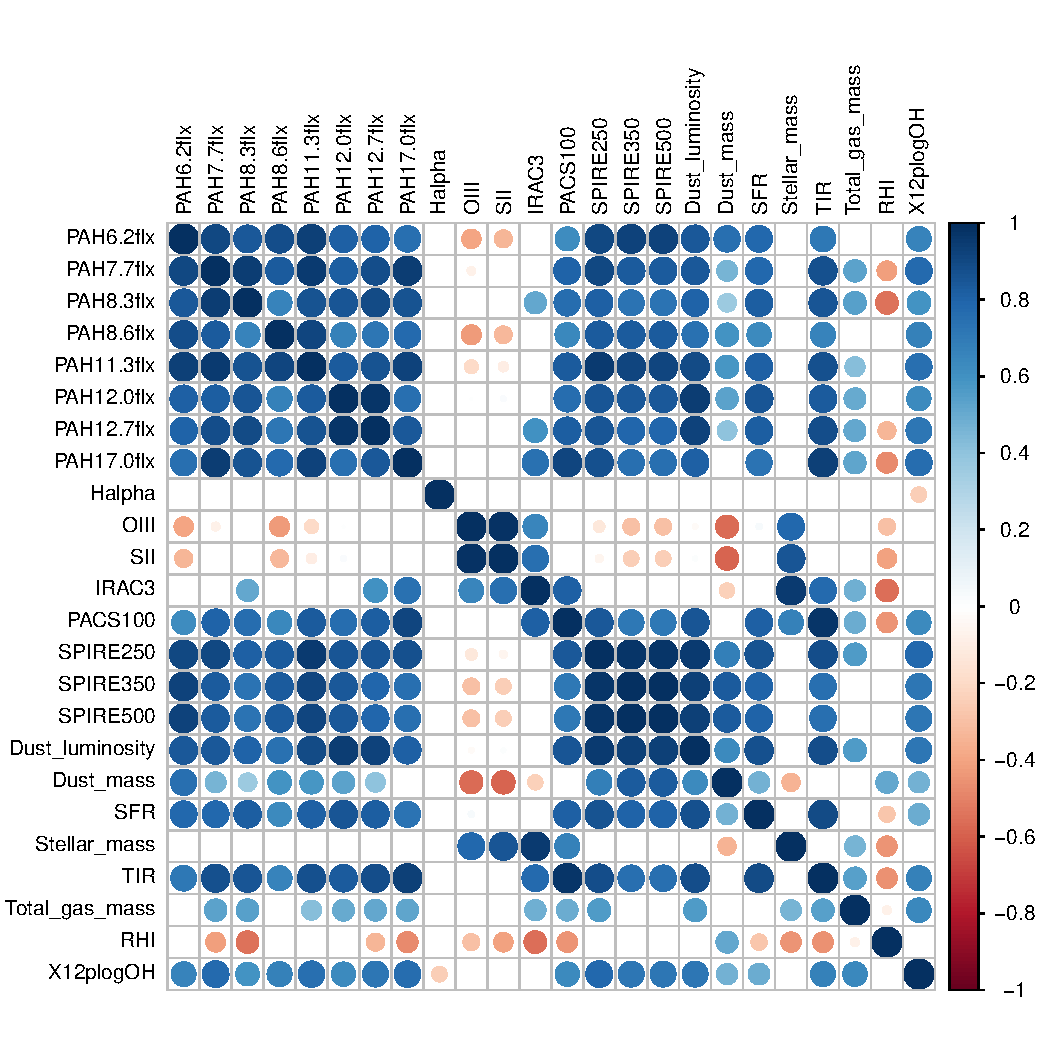
\includegraphics[width=\textwidth]{../images0.01/cor_plots/M31_all_derived_ones_core_plot_for_paper.pdf}
            \caption{Pearson correlation coefficients with a confidence level of 95 per cent for all data from M31. The colours and circles' size show the Pearson correlation coefficients where large blue circles are 1 which means highly correlated and large red circles are$-1$ means highly anti-correlated quantities. The non-significant correlations were left empty.}
            \label{fig: cor_all}
        \end{figure*}
 
